\section{Exercise 1}

In this problem, we'll analyze the execution of a code segment on a single-issue out-of-order processor.
\begin{figure}[H]
    \centering
    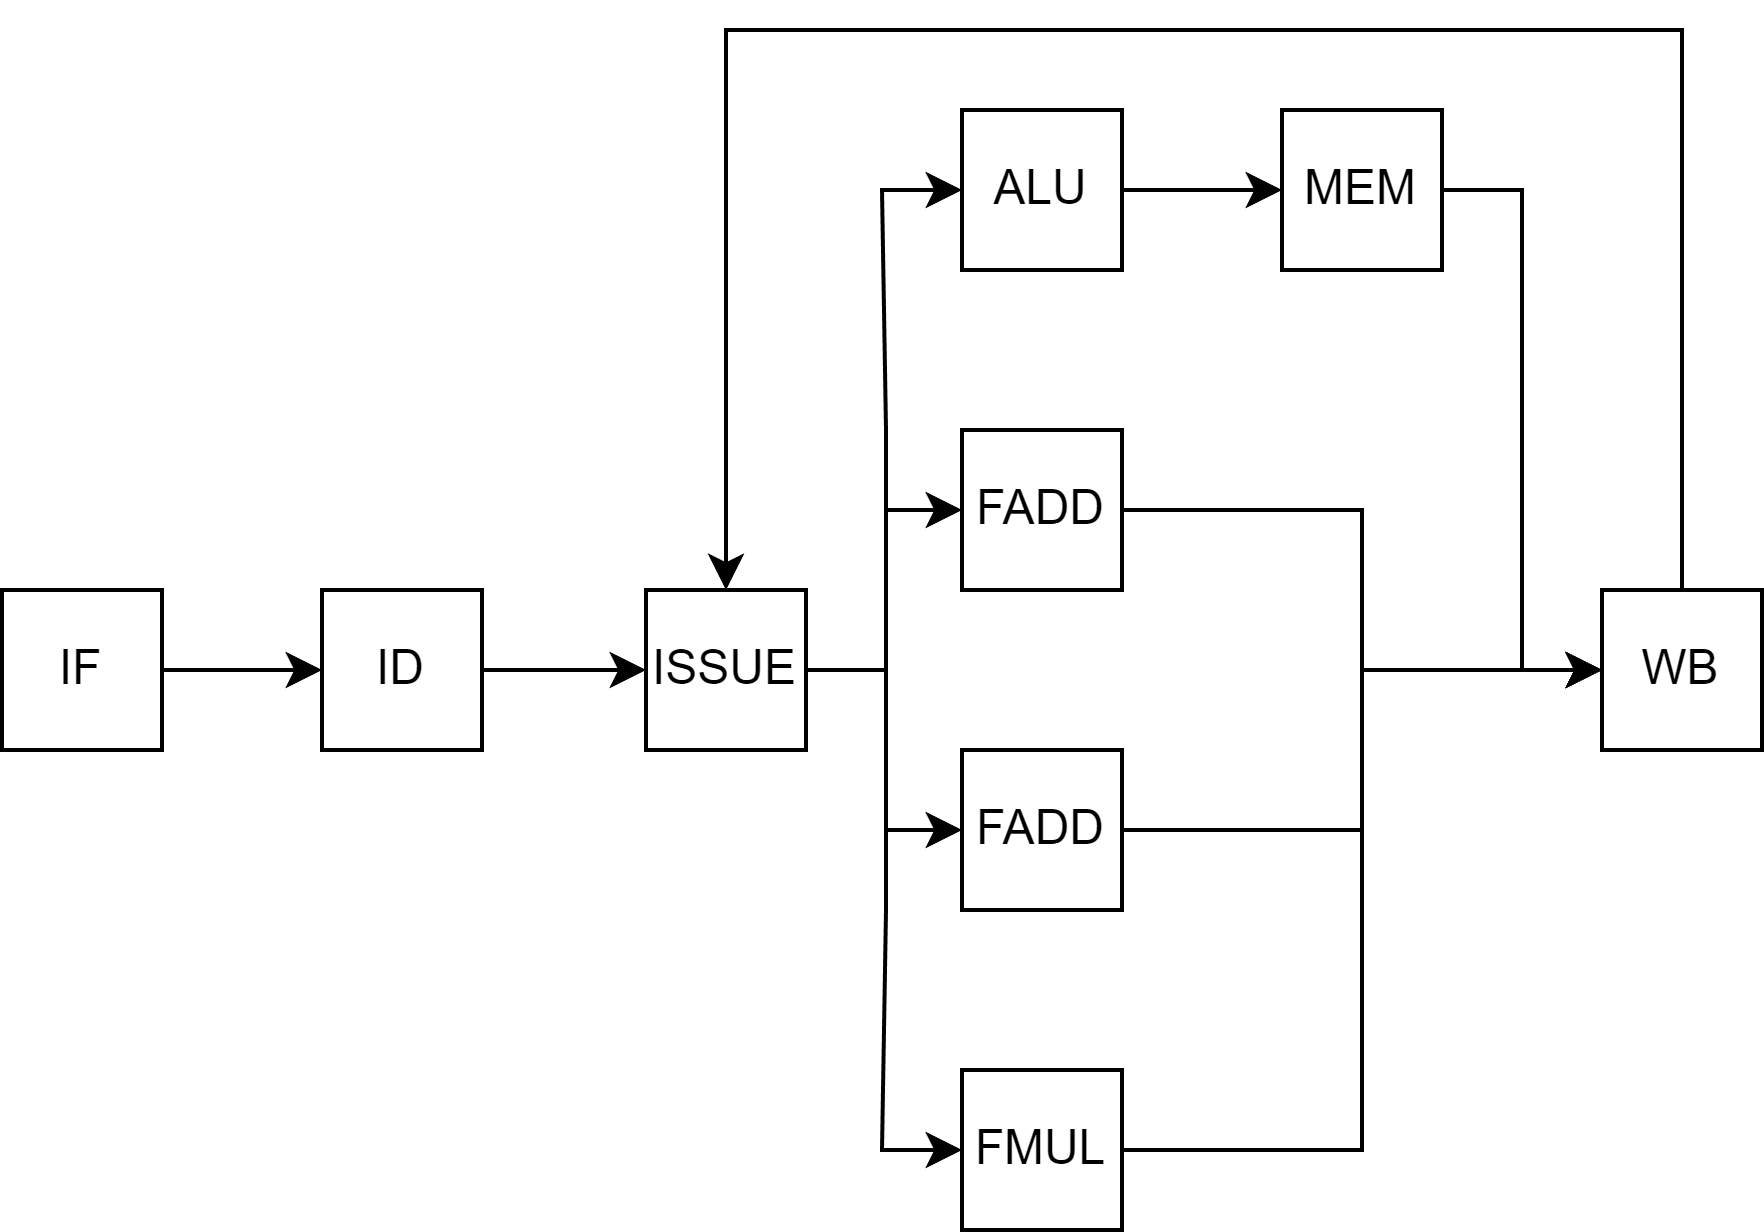
\includegraphics[width=0.75\linewidth]{images/complex.png}
\end{figure} 
Consider now the code:
\begin{verbnobox}[\verbarg]
LW F3,B(R0)
ADD F2,F2,F3
MUL F5,F4,F4
ADDI R0,R0,8
LW F3,B(R0)
ADD F2,F3,F5
\end{verbnobox}
Examine each conflict taking into account the following operation durations:
\begin{itemize}
    \item Arithmetic logic unit operations: one cycle.
    \item Memory operations: three cycles.
    \item Floating point addition: three cycles.
    \item Floating point multiplication: five cycles.
\end{itemize}

\subsection*{Solution}
The conflicts are: 
\begin{itemize}
    \item RAW R0 I4-I5.
    \item RAW F3 I5-I6.
    \item RAW F5 I3-I6.
    \item RAW F3 I1-I2.
    \item WAW F2 I2-I6.
    \item WAW F3 I1-I5.
    \item WAR F3 I2-I5.
    \item WAR R0 I1-I4. 
\end{itemize}
A possible execution is: 
\begin{table}[H]
    \resizebox{\textwidth}{!}{%
    \begin{tabular}{c|cccccccccccccccccccc}
    \textbf{Instruction} & \textbf{C1} & \textbf{C2} & \textbf{C3} & \textbf{C4} & \textbf{C5} & \textbf{C6} & \textbf{C7} & \textbf{C8} & \textbf{C9} & \textbf{C10} & \textbf{C11} & \textbf{C12} & \textbf{C13} & \textbf{C14} & \textbf{C15} & \textbf{C16} & \textbf{C17} & \textbf{C18} & \textbf{C19} & \textbf{C20} \\ \hline
    \textit{1}           & F           & D           & IS          & E1          & E2          & E3          & W           &             &             &              &              &              &              &              &              &              &              &              &              &              \\
    \textit{2}           &             & F           & D           & \underline{S}     & \underline{S}     & \underline{S}     & IS          & E1          & E2          & E3           & W            &              &              &              &              &              &              &              &              &              \\
    \textit{3}           &             &             & F           & \underline{S}     & \underline{S}     & \underline{S}     & D           & IS          & E1          & E2           & E3           & E4           & E5           & W            &              &              &              &              &              &              \\
    \textit{4}           &             &             &             & \underline{S}     & \underline{S}     & \underline{S}     & F           & D           & IS          & E            & \underline{S}      & W            &              &              &              &              &              &              &              &              \\
    \textit{5}           &             &             &             &             &             &             &             & F           & \underline{S}     & D            & \underline{S}      & IS           & E1           & E2           & E3           & W            &              &              &              &              \\
    \textit{6}           &             &             &             &             &             &             &             &             & \underline{S}     & F            & \underline{S}      & D            & \underline{S}      & \underline{S}      & \underline{S}      & IS           & E1           & E2           & E3           & W           
    \end{tabular}%
    }
\end{table}
If we assume that the issue stage is a buffer with an unlimited capacity to hold instructions awaiting execution:
\begin{table}[H]
    \resizebox{\textwidth}{!}{%
    \begin{tabular}{c|cccccccccccccccccccc}
    \textbf{Instruction} & \textbf{C1} & \textbf{C2} & \textbf{C3} & \textbf{C4} & \textbf{C5} & \textbf{C6} & \textbf{C7} & \textbf{C8} & \textbf{C9} & \textbf{C10} & \textbf{C11} & \textbf{C12} & \textbf{C13} & \textbf{C14} & \textbf{C15} & \textbf{C16} & \textbf{C17} & \textbf{C18} & \textbf{C19} & \textbf{C20} \\ \hline
    \textit{1}           & F           & D           & IS          & E1          & E2          & E3          & W           &             &             &              &              &              &              &              &              &              &              &              &              &              \\
    \textit{2}           &             & F           & D           & \underline{S}     & \underline{S}     & \underline{S}     & IS          & E1          & E2          & E3           & W            &              &              &              &              &              &              &              &              &              \\
    \textit{3}           &             &             & F           & D           & \underline{S}     & \underline{S}     & \underline{S}     & IS          & E1          & E2           & E3           & E4           & E5           & W            &              &              &              &              &              &              \\
    \textit{4}           &             &             &             & D           & \underline{S}     & D           & \underline{S}     & \underline{S}     & IS          & E            & \underline{S}      & W            &              &              &              &              &              &              &              &              \\
    \textit{5}           &             &             &             &             & \underline{S}     & F           & \underline{S}     & \underline{S}     & \underline{S}     & D            & \underline{S}      & IS           & E1           & E2           & E3           & W            &              &              &              &              \\
    \textit{6}           &             &             &             &             &             &             & \underline{S}     & \underline{S}     & \underline{S}     & F            & D      & \underline{S}      & \underline{S}      & \underline{S}      & \underline{S}      & IS           & E1           & E2           & E3           & W           
    \end{tabular}%
    }
\end{table}